\chapter{MagicDrawToGamma plugin}\label{chap:contrib}

Ebben a fejezetben bemutatom a munkám során elkészített alkalmazást kitérve, az alapkoncepcióra, az elméleti és gyakorlati problémákra és megoldásaikra. Továbbá kitérek a fejlesztés során felmerülő szoftver-infrastruktúra és implementáció okozta komplikációkra.

\section{Koncepció}
Állapottérképek formális verifikációjának támogatása MagicDraw-ban, egy plug-in fejlesztésével lett megvalósítva. A plug-in függ a Viatra For MagicDraw-tól, ami lehetővé teszi modellek transzformációját Viatra segítségével. A plug-in legfontosabb funkciója MagicDraw modellek Gamma modellekké való transzformációja. A letranszformált Gamma nyelvű modelleket az keretrendszer kezelni tudja, a verifikáció elvégzéséhez az eszköznek csak egyes részei szükségesek. A megoldást a \ref{fig:used-gamma} ábra szemlélteti. A felhasználónak lehetősége van megkötések megfogalmazására a plugin-al és elvégezni a verifikációt és megtekinteni az eredményt azaz, hogy teljesülnek-e a megkötések vagy sem.

\begin{figure}[!ht]
	\centering
	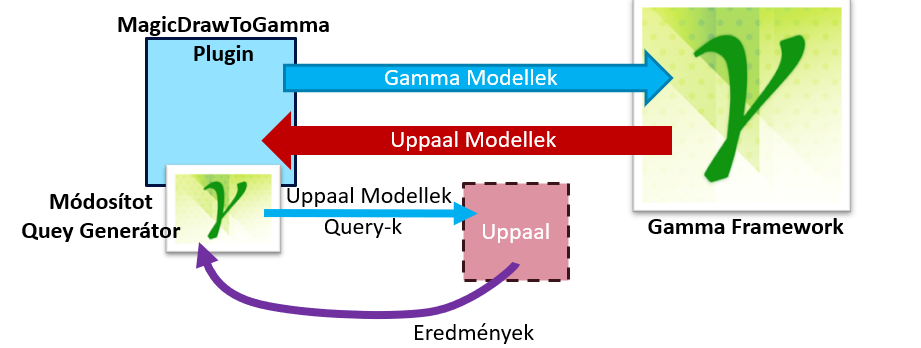
\includegraphics[keepaspectratio, width=150mm]{figures/concept.png}
	\caption{Koncepció}
	\label{fig:used-gamma}
\end{figure}

\section{Fejlesztőkörnyezet}
 A fejlesztés megkezdéséhez szükséges volt összeállítani egy olyan fejlesztőkörnyezetet amivel hatékonyan lehet plug-int fejleszteni. MagicDraw biztosít egy ún. \emph{skeletont} Eclipsehez és IntelliJhez is plug-in fejlesztéséhez, de a fejlesztés nem ezek segítségével hanem az IncQueryLabs által készített skeleton felhasználásával valósult meg. Ennek oka, hogy a hivatalos \emph{skeletonok} nem vagy csak részben működtek, a mögöttes infrastruktúra megismerése és javítása pedig túl hosszadalmas és a feladat szempontjából irreleváns lett volna. 
 
A skeleton egy Eclipse project, viszont Gradlet használ a projekt fordításához és a dependenciák kezeléséhez. Ez sokszor inkonzisztenciákhoz vezetett az egyik legnagyobb probléma a Viatra Querik generálása amiket csak Eclipsel lehet generálni. A kódbázis egy része nem Javában hanem Xtendben íródott, a Viatra modell transzformációk implementálása ezzel a nyelvvel egyszerűbb. Azok az osztályok melyeknél nem volt indokolt, jellemzően a MagicDraw felhasználói felületeinél, azok Java 8-ban lettek implementálva.

A dolgozat elkészítése idején a MagicDraw 19-es verziója is elérhető volt a plug-in azonban még nem ehhez, hanem a 18.5-ös verziójához készült. A kódbázis azonban kompatibilis lehet még az újabb verziókkal is, amennyiben az állapottérképeket érintő meta-modellek nem változnak.

Gamma(2.0) a verifikációt Uppaal segítségével végzi el. Ehhez előállít egy formális leírást a rendszerről és egy \emph{query}-t ami a rendszerrel szemben támasztott követelményeket írja le. A követelmények megírásához biztosít egy UI elemet amivel a felhasználó az Uppaal ismerete nélkül is képes a követelmények definiálására. Ez a funkció teljesen át lett emelve Gammából módosított implementációval a MagicDrawToGammába. A Gamma az Uppaalra az operációs rendszeren keresztül hív át, ezért az Uppaalt külön kell telepíteni és konfigurálni.

\section{MagicDraw - Gamma transzformáció}

A MagicDraw - Gamma transzfromációt egy menü elemmel lehet elindítani. Ehhez szükséges, hogy a projekthez hozzá legyen rendelve egy külső könyvtár (Gamma Workspace) ami a leképzett és perzisztensen eltárolandó modellek helyét jelöli. A hozzárendelt könyvtár abszolút elérését String formában a projekt tárolja, emiatt sem a projekt nem migrálható, sem pedig maga a Gamma Workspace. Továbbá a könyvtár karbantartása ebben a verzióban még a felhasználó felelőssége, ugyanis a plug-in nem töröl a könyvtárból csak hozzáad és módosít, ennek akkor van jelentősége, ha leképzés után egy állapottérkép el lett távolítva a MagicDraw modellből és utána újra le lett képezve. Ebben az esetben a régebben leképzett Gamma állapottérképek is megmaradnak.

\subsection{Gyökér elemek létrehozása:}

A plugin a transzformáió kezdetekor létrehoz egy \emph{ResourceSet}-et, amivel készít egy \emph{Resource}-t a \emph{Gamma Workpace} gyökerébe .s.md2g néven, továbbá egy Resource-t \verb+interfaces.gms+ néven. Az előbbi Resource egy segédstruktúrát tartalmaz ami a leképzett elemek visszakereshetőségéül szolgál (ld. \refstruc{sec:trace_model}), utóbbi pedig a modellben definiált interfaceket tárolja.

Az eszköz ezután Viatra Queryk segítségével megkeresi az állapotgépeket a MagicDrawban és végig iterál rajtuk. Minden állapottérképen kigyűjti az éleken használt \emph{SignalEventek}et és létrehoz a \emph{Signal}éval azonos néven egy Eventet a Gamma meta-modelljének megfelelően. Ez az Event a \emph{Signal} Gammabeli megfelelője.  A létrehozott eventek egy Interfacen kerülnek definiálásra aminek a neve megegyezik az állapottérképével. Az interface ezután belekerül az interfaceket tároló \emph{Resourceba}. Az eventek iránya INOUT ez lehetővé teszi, hogy az állapotképek küldhessenek és fogadhassanak.

A leképzett állapottérképek külön Resourceokba kerülnek amik a Gamma Workspace-ben egy külön az állapottérkép nevével megegyező könyvtárba kerülnek, ugyan ezen a néven .gsm kiterjesztéssel (\ref{fig:filestructure}-es ábra). (A Resource gyökere nem egy StatechartDefinition, hanem egy Package, ennek a neve szintén megegyezik az állapottérkép nevével)

\begin{figure}[H]
	\centering
	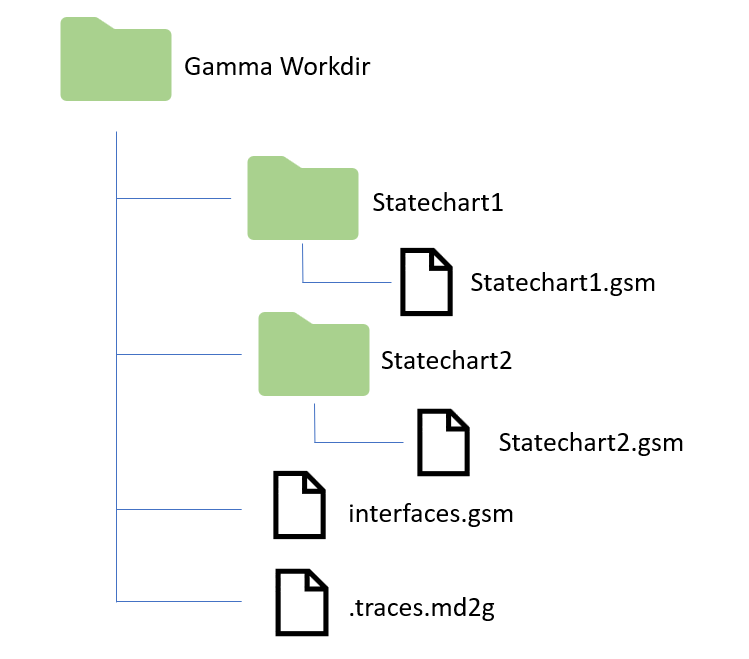
\includegraphics[keepaspectratio, width=90mm]{figures/filestructure.png}
	\caption{Létrehozott fájlstruktúra}
	\label{fig:filestructure}
\end{figure}

\subsection{Alap struktúra kialakítása:}

Az előző lépések során azok az elemek állnak elő, melyek a modellek gyökér elemeiként fognak szolgálni. A következő lépés létrehozni az állapottérképek egy belső, alap struktúráját, amit az állapotok és állapotátmenetek határoznak meg. A Viatra for MagicDraw projekt megnyitásakor készít egy ViatraQueryEngine-t aminek a \emph{Scope}-ja a megnyitott modellre terjed ki. A transzformációs szabályok regisztrálása ezen az engine-en történik, létrejön azonban még egy aminek a \emph{Scope}-ja magába foglalja az első lépésben létrehozott \emph{Resource}okat és a MagicDraw modellt is. A készülő modellben történő keresések, és a visszakövetések ezzel az \emph{engine}-el történnek. Alap struktúra kialakításának lépcsői:

\begin{enumerate}
	\item Fő régiók leképzése (olyan régió aminek a szülője állapotgép).
	\label{enum:elso}
	\item Régiókban található állapotok leképzése.
	\label{enum:masodik}
	\item Állapotokban található régiók leképzése.
	\label{enum:harmadik}
\end{enumerate}


A második lépésben a \emph{Trace Modell} alapján megkeressük a már leképzett régiót a Gamma Modellben és beletesszük az újonnan létrehozott és a MagicDraw modellnek megfelelően elnevezett állapotot, ha a régió még nincs leképezve akkor létrejön, és abba kerül bele az állapotot. Ez a lépés olyan részgráfokat is eredményezhet amikbe nem vezet út a gyökér elemekből. Ennek kiküszöbölése a harmadik. lépés ami, ugyanezt a műveletet hajtja végre csak a másik irányból, tehát az állapotok párjait keressük meg, amikbe régiókat helyezünk el. Ezek a régiók már létezhetnek ilyenkor nem új régió jön létre hanem a már meglévő kerül az állapotba. A működés során a MagicDraw modell jól formáltsága kihasznált és elvárt, továbbá az is ki van használva, hogy régió csak \emph{State}ben és \emph{StateMacine}-ban lehet. A régiókat tartalmazó állapotok kompozit és ortogonális állapotnak tekintendők.

A tartalmazási gráf összefüggővé válását \aref{fig:state-transformation} ábra szemlélteti.

\begin{figure}[H]
Az irányított nyilak tartalmazást jelölnek, a bekeretezett téglalap \emph{StatechartDefinition}, a szaggatott vonallal körbevett \emph{Region} és a körök \emph{Statek}.

\centering
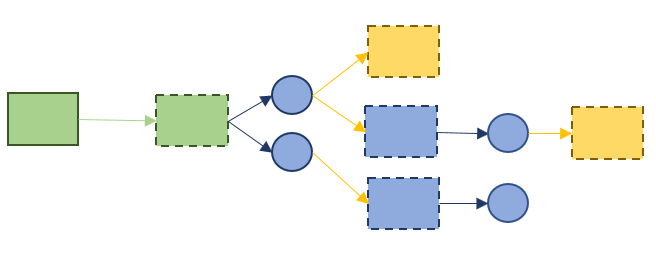
\includegraphics[keepaspectratio, width=140mm]{figures/transformation.png}
\caption{Állapotok és régiók leképzésének menete, \ref{enum:elso}. lépcső: zöld, \ref{enum:masodik}. lépcső: kék, \ref{enum:harmadik}. lépcső: sárga}
\label{fig:state-transformation}
\end{figure}

\subsection{Pszeudoállapotok átalakítása:}
Az állapotátmenetek leképzése előtt a pszeudoállapotok kerülnek leképzésre. Ezen a ponton már létezik minden régió amit tartalmazhatja őket. A leképzés legtöbb esetben támogatott viszont, egyes elemek tartalmazása esetén nem lehet a verifikációt végrehajtani. Az elemeket és párjaikat \aref{table:pseudo} táblázat mutatja.

\begin{table}[!h]
	\footnotesize
	\centering
	\begin{tabular}{ l c c }
		MagicDraw & Gamma & verifikálható \\ \hline
		InitialState & InitialState & igen \\
		Chioce & Choice & igen \\
		Junction & Merge & nem \\
		Fork & Fork & nem \\
		Join & Join & nem \\
		TerminalState & nincs & - \\
		Conn. PointReference & nincs & - \\
		EntryPoint & nincs & - \\
		ExitPoint & nincs & -
		
	\end{tabular}
	\caption{Pszeudoállapotok párosítása.}
	\label{table:pseudo}
\end{table}

\subsection{Állapotátmenetek leképzése:} A következő lépés az állapotátmenetek átalakítása. Ezen a ponton már az összes olyan elem leképzésre került, amely az állapotátmenetek kezdő, vagy végpontjaként szolgálhat. Egy MagicDraw modellben az állapotátmenetek régiók tartalmazzák, szemben Gammával, ahol a StatechartDefinition közvetlen gyerekei. A tartalmazó-tartalmazott, Statemahcine - Tranisiton párok megkeresése a következő patternekkel történik.
\lstset{style=VQL}
\begin{lstlisting}
pattern RegionsInRegion(container: Region, region: Region){
	Region.subvertex(container, vertex);
	State.region(vertex, region);
}
pattern RegionsInStatemachine(stateMachine: StateMachine, subregion: Region){
	find MainRegions(stateMachine, subregion);
} or {
	find RegionsInRegion+(region, subregion);
	StateMachine.region(stateMachine, region);
}
pattern TranisitonsInStateMachine(stateMachine: StateMachine, transition: Transition){
	find RegionsInStatemachine(stateMachine, region);
	Region.transition(region, transition);
}
\end{lstlisting}

A \emph{StateMachine} Gamma modellbeli párját a \emph{Trace modell} segítségével lehet megtalálni és hozzáadni a megfelelő állapotátmenetet.

Az átmenetek leképzése után már elérhetőséget lehet is vizsgálni.

\subsection{Változók leképzése}
Változókat MagicDraw-ban attribútumként lehet definiálni. Ezeknek a következő tulajdonságait lehet beállítani: láthatóság, típus, statikusság, alapértelmezett érték.

A láthatóság és a statikusság, a jelen verzióban nem bírnak jelentőséggel, hiszen minden állapottérkép \emph{singleton}nak tekinthető és egymástól független léteznek. A típus lehet bármilyen beépített vagy felhasználó által definiált típus vagy valamilyen primitív. A leképzés során kétféle primitív típus támogatott: \emph{Integer} és \emph{Boolean}, egyéb típusok leképzése még nem támogatott. A változók tulajdonságaira vonatkozó megkötéséket \aref{table:variables} táblázat foglalja össze.

\begin{table}[!h]
	\footnotesize
	\centering
	\begin{tabular}{ l r }
		Tulajdonság & Lehetséges érték\\ \hline
		Name & tetszőleges, de egyedi az állapotgépben\\
		Type & Integer, Boolean\\
		Static & tetszőleges, de mindig statikusnak tekintendő\\
		Visibility & tetszőleges, de mindig private-nak tekintendő
	\end{tabular}
	\caption{Változók lehetséges értékei.}
	\label{table:variables}
\end{table}



\subsection{Események, triggerek leképzése:} A MagicDrawban definiálható \emph{Triggerek} pontosabban az őket kiváltó események közül jelenleg kettő támogatott. Egyik a \emph{SignalEvent} a másik pedig \emph{TimeEvent}. Előbbi \emph{EventTriggerre} képződik le. A felhasználónak a \emph{SignalEvent} forrásával most még nem kell foglalkoznia, hiszen ezekhez automatikusan generálódik egy \emph{Interface} és egy \emph{Port}.

A \emph{Time Eventek} MagicDraw-ban kétféle típusúak lehetnek: relatív és abszolút. Utóbbit a plugin-in még nem támogatja.
A relatív típusú \emph{Time Eventek} a Gamma \emph{Timeout} mechanizmusának feleltethető meg. Ez három részből áll: \emph{StatechartDefinition}-ön definiált \emph{TimeoutDeclaration}, akció ami ennek beállítja az értékét (ami lehet szekundumban, vagy milliszekundumban mért) és maga a \emph{Trigger} ami hivatkozik a deklarációra. A \emph{TimeoutDeclaration} és az érték beállítása implicit történik a felhasználónak az időt kell megadnia trigger felvételekor a MagicDraw modellben.

\subsection{Őrfeltételek leképzése:}
Őrfeltételek definiálása MagicDraw állapottérképeken Opaque Expressionökkel\footnote{Szöveges nyelvel leírt kifejezés} történik, ezért ezt le kell fordítani és modell alapú leírássá konvertálni. Kifejezéseket Gammában a Constraint modellel lehet leírni. Ehhez tartozik egy nyelvtan is ami Xtext segítségével képes a Gamma Constraint nyelvből EMF alapú \emph{Constraint} példánymodellt fordítani.

A leképzéshez a \emph{Constraint Model Expressio}n szabálya lett felhasználva, amely alapján az Xtext parser előállítja a szöveges bemenetből a megfelelő \emph{Expression} példányt.
\lstset{style=javacode}
\begin{lstlisting}
Injector injector = new StatechartLanguageStandaloneSetup()
						.createInjectorAndDoEMFRegistration();
						
ParserRule rule = injector.getInstance(StatechartLanguageGrammarAccess.class)
						.getExpressionRule();
						
IParseResult result = injector.getInstance(StatechartLanguageParser.class)
						.parse(rule, new StringReader(guardString));
\end{lstlisting}

A referenciák viszont nem lesznek feloldva ezért ezek feloldása \emph{VIATRA} segítségével utólagosan történik a deklarációk név szerinti megkeresésével az előálló Gamma modellekből.
\lstset{style=VQL}
\begin{lstlisting}
pattern DeclarationsByName(statechartDefinition: StatechartDefinition, name: java String, declaration: Declaration){
	StatechartDefinition.variableDeclarations(statechartDefinition, declaration);
	Declaration.name(declaration, name);
}
\end{lstlisting}
 Mivel az őrfeltételek megírása a gamma nyelvével történik azért ugyan azokat az operátorokat támogatja, mint a gamma.

\begin{table}[!h]
	\footnotesize
	\centering
	\begin{tabular}{ l l l l }
		Név & Operátor& leírás & Csoportosítás \\ \hline
		 Imlikáció & imply & implikáció & jobbról balra \\
		 Diszjunkció & or & logikai vagy & n-szeres\\
		 Konjunkció & and & logikai és & n-szeres \\
		 Negálás & not & logikai nem & jobbról balra \\
		 Egyenlőség & =, /= & egyenlőség, egyenlőtlenség & jobbról balra \\
		 Reláció & <, >, <=, >= & relációs operátorok & balról jobbra \\  
		 Hozzáadás & +, - & hozzáadás, kivonás & balról jobbra \\
		 Skálázás & *, / & szorzás, osztás & balról jobbra \\
		 Maradék & mod & maradékos osztás & balról jobbra \\
		 Egész osztás & div & egész osztás & balról jobbra \\
		 Előjel & +, - & egyváltozós +, egyváltozós - & balról jobbra
	\end{tabular}
	\caption{Támogatott operátorok.}
	\label{table:operators}
\end{table}


\subsection{Akciók leképzése:}
Az akciók viselkedések amiket négyféle helyen lehet végrehajtani egy állapottérképen:

\begin{enumerate}
	\item Állapotvátáskor: a viselkedés állapotváltáskor hajtódik végre.
	\item Állapotba való belépéskor (\emph{Entry}): a viselkedés akkor hajtódik végre amikor az állapot aktívvá válik.
	\item Állapotban maradva (\emph{Do}): a viselkedés addig hajtódik végre amíg az állapot aktív.
	\item Állapotból kilépve (\emph{Exit}): a viselkedés állapotból való kilépéskor hajtódik végre.
\end{enumerate}

A MagicDraw akciói viselkedések (\emph{Behavior}) lehetnek: pl. \emph{StateMachine}, \emph{Activity}, \textbf{OpaqueBehavior}. Az OpaqueBehavior pontosabban ennek egy része az OpaqueExpression lehetővé teszi, hogy valamilyen szöveges szintaxissal írjunk le viselkedést. Ennek felhasználásával, hasonlóan az őrfeltételek esetében Xtext segítségével elő tudjuk állítani a megfelelő EMF modellt a Gamma szintaxisa szerint. Ehhez a \verb+ActionRule+ szabályra van szükség.

Jelenleg kétféle akció támogatott: értékadás és az eseményküldés. Ezek szintaxisa az alábbi:

\begin{lstlisting}
	//assignment action
	variableName := 1;
	//raise event action
	raise All.Event
\end{lstlisting}

Az \emph{All} nem Gamma specifikus jelölése az össze portnak, ebből jelenleg csak egy van egy implicit generált az események fogadáshoz, így jelen esetben az \emph{All} megjelölés csak ezt a portot választja ki.

\subparagraph{Megjegyzés:} a küldött eseményeknek nincs hatása, nem fogadja őket az állapottérkép, még akkor sem ha az interfészén az eseemények \emph{INOUT}-ként vannak definiálva.

\subsection{Trace Modell}
\label{sec:trace_model}
A leképzések végrehajtása során fontos követni, hogy mely elemek képződtek le és mely elemekké. Erre a célra a MagicDrawToGamma bevezet egy Trace modell\footnote{Nem összekeverendő a \aref{sec:formal-verif} fejezetben említett \emph{Execusion Tracel}} nevű segédstruktúrát, ami lehetővé teszi a megfeleltetések visszakereshetőségét VIATRA segítségével, továbbá a modell sorosítása és háttértáron való tárolása is megoldott. A modell EMF-ben van definiálva és  háromféle \emph{Trace}-t különbötet meg. Az Gamma állapottérképek alap elemeit \verb+Trace+-ek, az interfészek elemeit \verb+InterfaceTrace+-k és a \emph{Contraint} modell elemeit \verb+ConstraintTracek+ kötik össze MagicDraw párjukkal, amiből le lettek képezve.

A három \verb+Trace+ típust egy \verb+AbstractTrace+ osztály fogja össze, és \verb+MD2GTrace+-ben tárolhatók. (\ref{fig:trace-model} ábra)

\begin{figure}[ht]
	\centering
	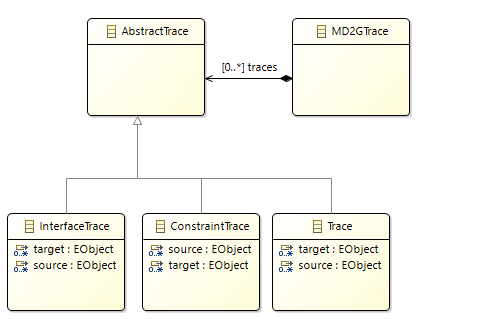
\includegraphics[keepaspectratio, width=140mm]{figures/trace-model.png}
	\caption{Trace modell EMF definíciója}
	\label{fig:trace-model}
\end{figure}


\section{A Verifikáció végrehajtása}
A verifikáció végrehajtásához két dologra van szükség. A modellnek egy leírására amit az Uppaal képes értelmezni és előállítani egy időzített automatát belőle és az Uppaal Query nyelvén megfogalmazott feltételekre. A MagicDrawToGamma kétféle lehetőséget biztosít a verifikáció végrehajtására.

\begin{enumerate}
	\item Uppaal közvetlen használata
	\item Uppaal Query Generator
	\label{en:fels}
\end{enumerate}

Első lehetőség időzített automaták leírásának előállítása amit a felhasználó megnyithat \emph{UPPAAL}-al. Ennek végrehajtása két részből áll. Először a Gamma modellt át kell alakítani, ez a \verb+StatechartToUppaalTransformer+ osztályon keresztül történik, ami a Gamma része.
\begin{lstlisting}
//initialize with a Gamma Package
StatechartToUppaalTransformer transformer = new StatechartToUppaalTransformer(p);
SimpleEntry<NTA, G2UTrace> entry = transformer.execute();
\end{lstlisting}
Ennek a kimenete két EMF alapú modell, egy \emph{trace modell} (\verb+GU2Trace+) és egy időzített auto
mata (\verb+NTA+). Az \textbf{időzített automata}\footnote{a formális verifikáció az időzített autómaták formalizmusán törénik} modelljét ezután egy formális leírásként kell szerializálni amit az UPPAAL képes beolvasni. Ez a Gamma \verb+UppaalModelSerializer+ osztálya állítja elő. 
\begin{lstlisting}
//NTA, parentFolder, fileName
UppaalModelSerializer.saveToXML(entry.getKey(), selected.getPath() , name +".xml");
\end{lstlisting}
A kimenetek a \emph{Gamma Workspace-ben} az állapottérkép könyvtárába kerülnek, ahonnan a felhasználó megnyithatja őket \emph{UPPAAL}-ban.

A második lehetőség az \emph{Uppaal Query Genertor} (\ref{fig:upp-query-gen} ábra) használata. Ez egy segédablak amivel a felhasználó egy grafikus felhaszálói interfészen tud \emph{UPPAAL Query}-ket definiálni, így a felhasználónak nem szükséges elsajátítania az \emph{UPPAAL Query}-k szintaxisát.

\begin{figure}[!ht]
	\centering
	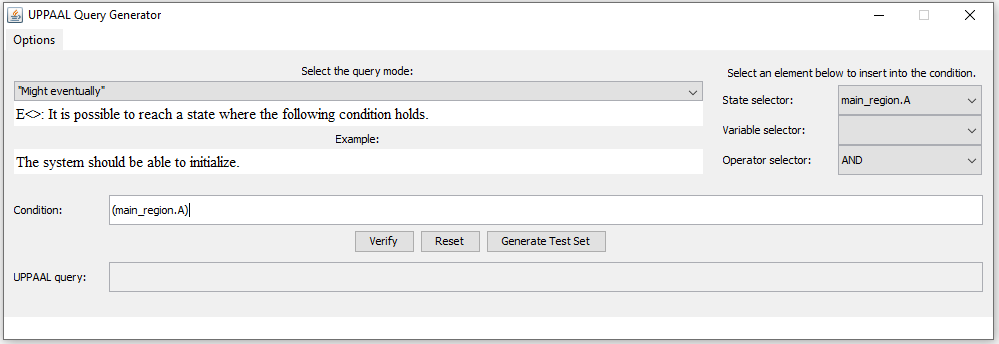
\includegraphics[keepaspectratio, width=150mm]{figures/query-gen.png}
	\caption{UPPAAL Query Generator}
	\label{fig:upp-query-gen}
\end{figure}

A Query Generátor implementációja a Gammából át lett emelve a MagicDraw plug-inba és az implementáció módosítva lett, hogy ebben a környezetben is tudjon működni. A Gamma egyik funkciója, hogy a formális verifikáció során esetleg keletkező ellenpéldákból képes Java nyelvű teszteseteket és szimulációt generálni Yakinduhoz. A MagicDrawToGammában a kódgenerálást még nem támogatja és a modellek nem Yakinduból származnak ezért ez a funkció nem használható a jelenlegi verzióban.

\section{Esettanulmány}

Az előző alfejezetek a MagicDrawToGamma főbb funkcióinak ismertetéséről és a funkciók megvalósítását mutatták be. Ebben az alfejezetben a  tényleges működéséről lesz szó egy példán keresztül.

\subsection{Szemléltető példa}

\paragraph{Példa specifikációja:} egy munkagépbe valamilyen anyagot lehet tölteni amit a gép tíz másodperc alatt feldolgoz. A gép az első bekapcsoláskor előbb szerviz állapotba kapcsol, ilyenkor kinyílik egy ajtó ami a gép szervizelését teszi lehetővé. Ahhoz, hogy a munkafolyamat elindulhasson a gépet üzem állapotba kell helyezni. Ilyenkor a gép ajtaja becsukódik és egy jel hatására feldolgozza a bemenetén elhelyezett anyagot. A gép kikapcsolásnál megjegyzi hogy szerviz vagy üzem állapotban volt-e és abba kapcsol vissza.

\paragraph{Rendszer állapot alapú definíciója:} A rendszer két jól megkülönböztethető állapotból áll \verb+Acitve+ és \verb+Inactive+. Az \verb+Active+ állapot felbontható két belső állapotra, hogy szerviz vagy üzem módba van: \verb+Maintentece+, \verb+Operation+. Ezeken kívül bevezethető még két állapot, hogy feldogoz-e épp anyagot a rendszer vagy sem: \verb+Idle+, \verb+Processing+. \verb+Maintenance+ állapotban a \verb+Processing+ állapotba való belépést egy logikai változóval \verb+enabled+ tiltjuk és engedélyezzük. Ezek alapján a rendszer egy lehetséges leírása lehet:
\begin{figure}[H]
	\centering
	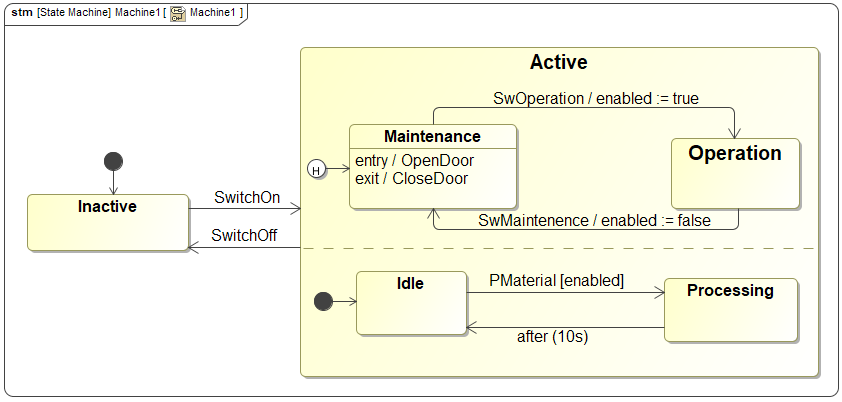
\includegraphics[keepaspectratio, width=150mm]{figures/machine1.png}
	\caption{Lehetséges leírás}
	\label{fig:leiras}
\end{figure}
\subparagraph{Megjegyzés} Az \verb+OpenDoor+ és \verb+CloseDoor+ akciók csak szemléltetés jellegűek, ezek nem kerülnek leképzésre.
\subparagraph{Feladat:} Ellenőrizzük, hogy a \verb+Maintentance+ és \verb+Processing+ állapotok kizárják egymást. Azaz a rendszer ne kerülhessen olyan állapotba, hogy nyitva van az ajtó miközben még feldolgoz a rendszer, hiszen ez veszélynek tenné ki a dolgozókat.
\subsection{Verifikáció menete}
Ahhoz, hogy le tudjuk ellenőrizni, hogy a leírt működés megfelel-e a támasztott feltételeknek végre kell hajtanunk a MagicDraw - Gamma transzformációt. Ezt a MD2G menüpont alatt található \verb+Perform Gamma Transformation+ kiválasztásával lehet megtenni (\ref{fig:md2g} ábra).
\begin{figure}[H]
	\centering
	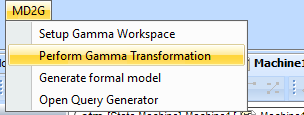
\includegraphics[keepaspectratio, width=70mm]{figures/GammaTrafo.png}
	\caption{MD2G menüpontok}
	\label{fig:md2g}
\end{figure}

A menüpontot kiválasztva előállíthatjuk az általunk kiválasztott Gamma Workspacebe a Gamma példánymodelleket, ez viszont önmagában még nem elég ezeket formális modellekké kell alakítanunk, hogy UPPAAL-al is fel lehessen őket dolgozni. Ezt a \verb+Generate formal model+ menüponttal tudjuk végrehajtani. Ez feldob egy könyvtárválasztó ablakot amiben a Gamma Workspace-ben található könyvtárak közül ki kell választanunk a megfelelő modellt tartalmazót (jelen példánál maradva a könyvtár nevem most Machine1 ez látható \aref{fig:leiras}. árán címkeként is).

A formális modell előállítása után a \verb+Open Query Generator+ menüponttal tudjuk megnyitni a \emph{Query Generator}-t, hasonlóan mint az előző lépésben ki kell választanunk újra a megfelelő könyvtárat a Gamma Workspace-ünkből, ami a formális modellt tartalmazza.

\paragraph{Feltétel megfogalmazása: } a feltétel amit megszeretnénk fogalmazni, hogy nem lehet a rendszer egyszerre \verb+Maintenance+ és \verb+Processing+ állapotban.
\[ \neg(Maintenance  \land Processing) = \neg Maintenance \lor \neg Processing \]
A kifejezést a Gamma \emph{Query Generátor}ba a következő alakba kell bevinnünk:
\begin{lstlisting}
	!(Active_1.Maintenance) || !(Active_2.Processing)
\end{lstlisting}
Ennek megírásához a \emph{Query Generator} segítséget nyújt a hivatkozható elemek és a köztük megfogalmazható relációk felsorolásával. A feltételtől azt várjuk, hogy mindig teljesüljön ezért a \verb+query mode+-ot \emph{Must Always}ra állítjuk. A verifikációt a \verb+verify+ gomb megnyomásával hajthatjuk végre az eredményt  \aref{fig:query-gen-res} ábra szemlélteti.
\begin{figure}[H]
	\centering
	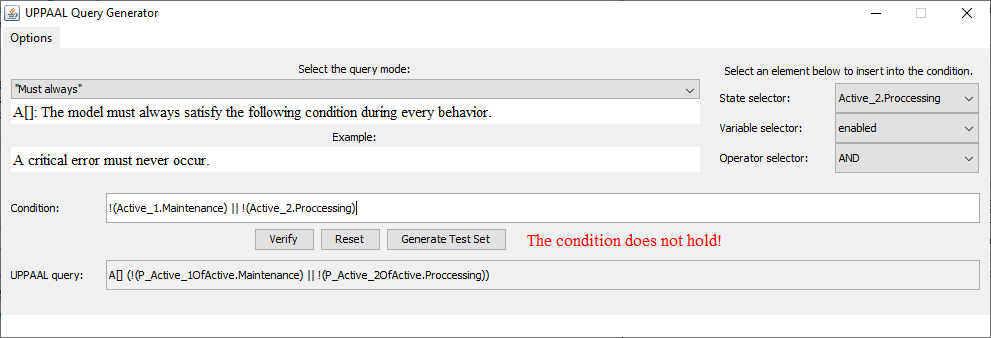
\includegraphics[keepaspectratio, width=150mm]{figures/query-gen-result.png}
	\caption{Verifikáció eredménye}
	\label{fig:query-gen-res}
\end{figure}

\paragraph{Eredmény:} A megszorítások nem teljesülnek, ennek okát sajnos a plug-in még nem képes levezetni, ezt nekünk kell kitalálni vagy az UPPAAL segítségével megnyithatjuk a formális modellt és az generált UPPAAL query segítségével azon belül is el tudjuk végezni a verifikációt és tanulmányozni a generált végrehajtási útvonalakat. Ehhez azonban az UPPAAL és a leképzések ismerete szükséges.
\subsection{A probléma:} A példa esetében a megszorítások megsértését a következő okozza: az állapotgép belép \verb+Operation+ állapotba, ilyenkor az ajtók zárva vannak a működés pedig engedélyezve. Megkezdődik a feldolgozás viszont mielőtt letelne a tíz másodperc a gépet szerviz állapotba kapcsolják így egyszerre lesz \verb+Maintenance+ és \verb+Processing+ állapotban amíg a feldolgozás maradék ideje le nem telik.

\begin{figure}[H]
	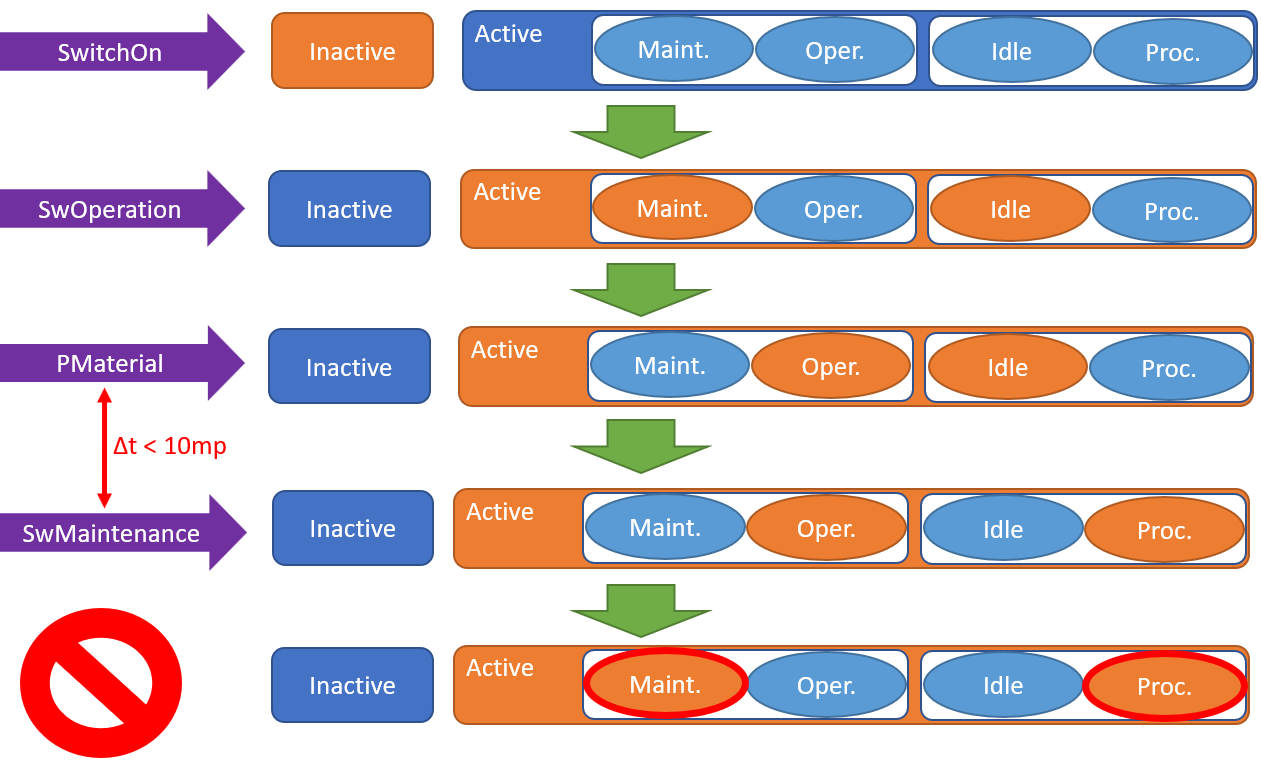
\includegraphics[keepaspectratio, width=150mm]{figures/trace.png}
	\caption{A megkötés megsértéséhez vezető út}
\end{figure}

\subsection{Megoldás}
Lehetséges megoldás lehet a probléma kiküszöbölésére egy köztes állapot bevezetése az \verb+Active+ ortogonális állapot felső régiójába. A gép szerviz állapotba kapcsoláskor előbb ide lép át, ilyenkor a feldolgozás letiltódik. Itt várakozik, méghozzá annyi időt, amennyi a feldolgozáshoz legalább szükséges. Ez a működés tehát megvárja a még folyamatban lévő feldolgozás befejezését és csak utána lép át a \verb+Maintenance+ állapotba. A módosított állapottérképet az új állapottal (\verb+Switching+) és a verifikáció eredményét \aref{fig:machine2}. ábra mutatja.
\begin{figure}[H]
	\centering
	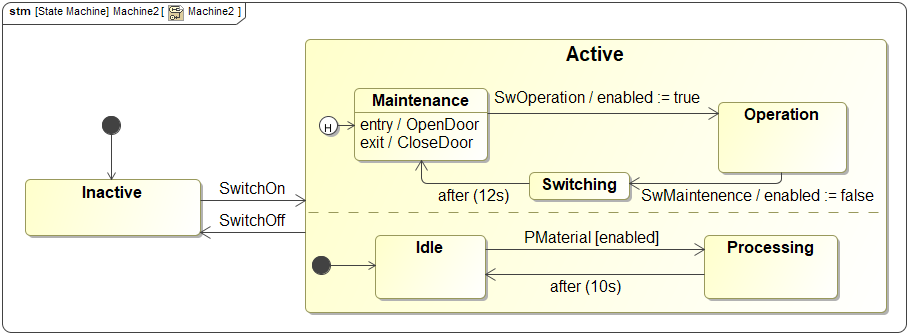
\includegraphics[keepaspectratio, width=150mm]{figures/machine2.png}
	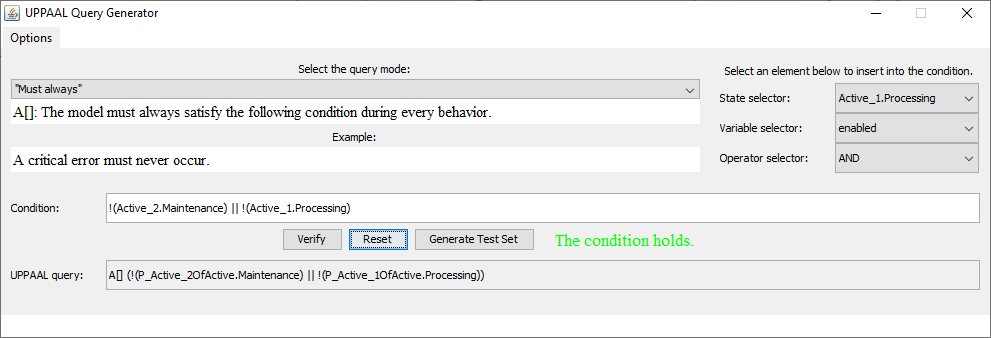
\includegraphics[keepaspectratio, width=150mm]{figures/fixed-result.png}
	\caption{Módosított állapottérkép és a verifikáció eredménye}
	\label{fig:machine2}
\end{figure}










